\section{HTTP}
\label{sec:http}

Das Hypertext Transfer Protocol (HTTP) ist ein Protokoll für die Kommunikation zwischen einem Web-Browser und einem Web-Server [\cite{http}]. Dabei folgt HTTP dem üblichen Client-Server Modell: Der Web-Browser, hier der Client (dt: Benutzer), eröffnet also die Verbindung und stellt eine Anfrage, der Server empfängt diese, und sendet daraufhin eine Antwort an den wartenden Client. Da der Server in der Kommunikation via HTTP keine Daten zwischen zwei Anfragen speichert, gilt dieses Protokoll als zustandslos. HTTP bildet die Grundlage von jedem Datenaustausch über das Web [\cite{httpUsage}].

Es werden jedoch verschiedene Standards dieses Protokolls benutzt. Zum Stand von November 2021 wird HTTP/2 zwar von etwa 97,59 \% der Browser unterstützt (gewichtet nach Marktanteil) [\cite{http2Browser}], aber nur von etwa 46,8 \% der 10 Millionen meistbesuchten Webseiten [\cite{http2Website}]. HTTP/3 ist die neuste aufkommende Version des Standards. Als wesentliche Veränderung zu den Vorgängern benutzt HTTP/3 das Netzwerkprotokoll QUIC statt dem Transmission Control Protocol (TCP) für die tieferliegende Kommunikation [\cite{http3}]. Die dritte Version von HTTP wird zum Stand vom November 2021 von 73,51 \% der Browser unterstützt [\cite{http3Browser}] und von 23,4 \% der meistbenutzten Webseiten [\cite{http3Website}].

\subsection{HTTPS}
\label{subsec:http_https}

HTTPS ist eine Erweiterung von HTTP, wobei die gesendeten Daten mittels Transport Layer Security (TLS) beziehungsweise früher mittels Secure Sockets Layer (SSL) verschlüsselt werden [\cite{https}]. Daraus folgt ein Schutz der Integrität und Vertraulichkeit der Daten zwischen dem Computer des Benutzers und dem angefragten Server. Die Telemetriedaten des Firefox Browsers zeigen an, dass im November 2021 etwa 82,62 \% der von Nutzern aufgerufenen Webseiten über HTTPS geladen wurden [\cite{httpsUsage}].\\
In Grafik \ref{fig:HTTPS} wird der übliche Nachrichtenverkehr einer HTTPS Verbindung zwischen einem Client (insbesondere einem Web-Browser) und einem Server dargestellt. Dabei ist ersichtlich, dass die Kommunikation im Wesentlichen in drei Schritte geteilt ist:

Schritt 1: TCP Verbindung aufbauen\\
Schritt 2: TLS Verschlüsselung herstellen\\
Schritt 3: Anfrage senden und Antwort erhalten
%
\begin{figure}[htbp]
	\centering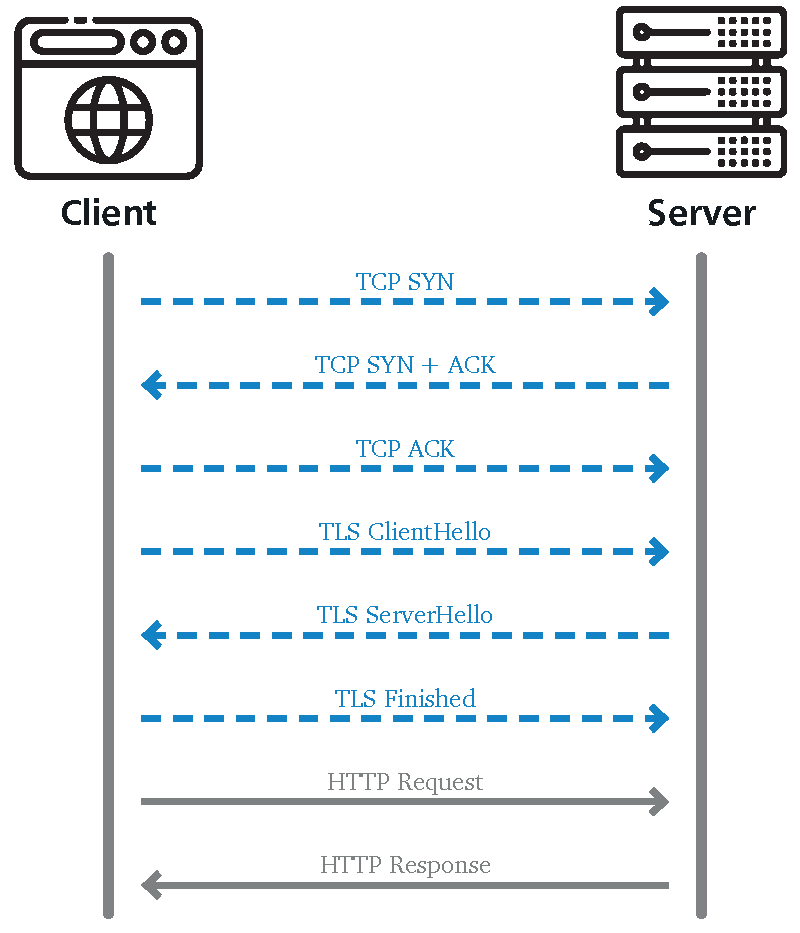
\includegraphics[width=0.7\textwidth]{images/03/HTTPS.pdf}
    \caption{HTTP Request Over TCP + TLS}
    \label{fig:HTTPS}
\end{figure}

\subsection{URI/URL}
\label{subsec:http_uri}

Ein Uniform Resource Identifier (URI) ist ein Bezeichner, welcher aus einer eindeutigen Reihenfolge von Zeichen besteht. 
Der Zweck eines URI ist es, eine Ressource eindeutig zu identifizieren [\cite{uri}].

Eine Unterform des URI ist der Uniform Resource Locator (URL), welcher eine Ressource nicht nur eindeutig identifiziert, sondern auch als eine Adresse zu dieser Ressource dient. Im Kontext des Internets werden in der Regel URLs von der Form \verb|https://robin-garbe.de/a/uni/BA-Thesis.pdf| genutzt. Eine URL kann jedoch erweitert werden. Dies wird oft genutzt, um auf eine untergeordnete Ressource oder auf einen spezifischen Teil der Ressource direkt zu verweisen. Die Grafik \ref{fig:URI} zeigt ein Beispiel für eine solche Erweiterung.
%
\begin{figure}[htbp]
	\centering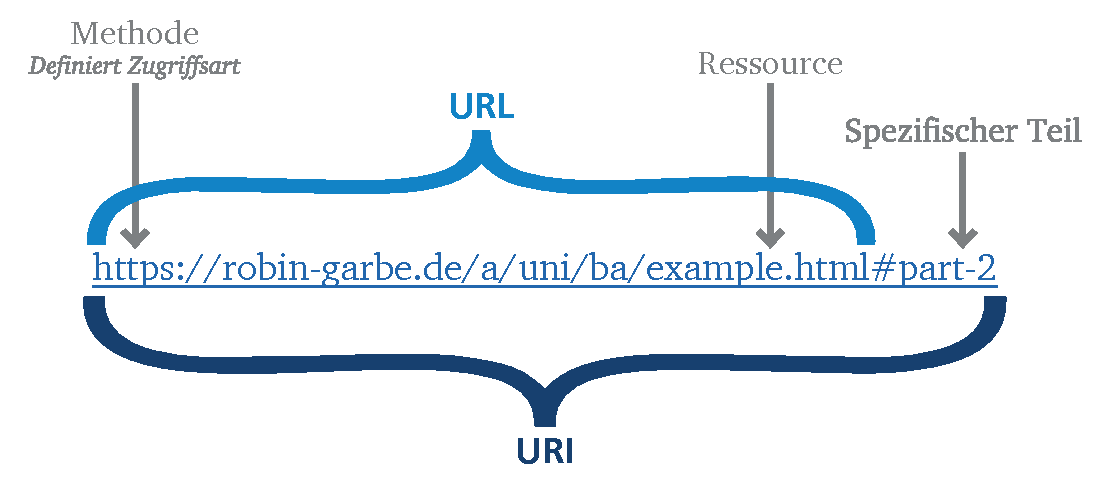
\includegraphics[width=0.85\textwidth]{images/03/URI.pdf}
    \caption{Extended URL Example}
    \label{fig:URI}
\end{figure}
